% ****** Start of file apssamp.tex ******
%
%   This file is part of the APS files in the REVTeX 4.1 distribution.
%   Version 4.1r of REVTeX, August 2010
%
%   Copyright (c) 2009, 2010 The American Physical Society.
%
%   See the REVTeX 4 README file for restrictions and more information.
%
% TeX'ing this file requires that you have AMS-LaTeX 2.0 installed
% as well as the rest of the prerequisites for REVTeX 4.1
%
% See the REVTeX 4 README file
% It also requires running BibTeX. The commands are as follows:
%
%  1)  latex apssamp.tex
%  2)  bibtex apssamp
%  3)  latex apssamp.tex
%  4)  latex apssamp.tex
%
\documentclass[%
 %reprint,
%superscriptaddress,
%groupedaddress,
%unsortedaddress,
%runinaddress,
%frontmatterverbose, 
%preprint,
%showpacs,preprintnumbers,
%nofootinbib,
%nobibnotes,
%bibnotes,
 amsmath,amssymb,
 aps,
%pra,
%prb,
%rmp,
%prstab,
%prstper,
floatfix,
aps,prd,longbibliography,
notitlepage
]{revtex4-1}

\usepackage{graphicx}% Include figure files
\usepackage{dcolumn}% Align table columns on decimal point
%\usepackage{bm}
\usepackage{multirow}
\usepackage{natbib}

\newcommand{\BE}{\begin{equation}}
\newcommand{\EE}{\end{equation}}
\newcommand{\figpath}{../Data/Data/Curves/}
\newcommand{\BV}{buoyancy }

\begin{document}

\preprint{APS/123-QED}

\title{Taylor-Couette Flow in the Classroom}


\author{Daniel Borrero}
\affiliation{Willamette University, Salem, Oregon 97301} 
 \email{dborrero@willamette.edu}
 
\author{Bruce Rodenborn}%
\email{bruce.rodenborn@centre.edu}
\affiliation{Physics Program, Centre College, Danville, KY 40422}
\date{\today}% It is always \today, today,
             %  but any date may be explicitly specified

\begin{abstract}


%\begin{description}
%\item[Usage]
%Secondary publications and information retrieval purposes.
%%\item[PACS numbers]
%%May be entered using the \verb+\pacs{#1}+ command.
%\item[Structure]
%You may use the \texttt{description} environment to structure your abstract;
%use the optional argument of the \verb+\item+ command to give the category of each item. 
%\end{description}
\end{abstract}

%\pacs{Valid PACS appear here}% PACS, the Physics and Astronomy
                             % Classification Scheme.
%\keywords{Suggested keywords}%Use showkeys class option if keyword
                              %display desired
\maketitle

%\tableofcontents

%\linespread{2}
\section{Introduction}

We present a low-cost fluid dynamics experiment that is useful in a variety of classroom contexts because it displays a rich variety of patterns that lend themselves to analysis at the undergraduate and graduate levels or even in a high-school physics class. The apparatus consists of concentric rotating cylinders with fluid in the gap between them, Fig. XX. The system can be constructed for under \$100 and the primary measurements are made using a webcam or other digital camera. Similar systems have been used successfully for over ten years at the Hands-On School in Complex Systems, which is a two-week winter school designed to teach low-cost experimental techniques to STEM faculty in developing countries sponsored by the International Center for Theoretical Physics in Trieste Italy.

\section {Background}
Fluid flow between rotating cylinders is typically called  Couette-Taylor flow after Maurice Couette who was a professor of physics at the University of Angers in France and English physicist and mathematician G.I. Taylor who studied the systems higher order instabilities in the 1920's\cite{couette_taylor}.  The system continues to be used as a viscometer, but it is also used for studies of the stability of rotating shear flows and and as a pedagogical tool in the classroom.

In 1888 Couette determined the viscosity of liquids from measurements of the torque for laminar flow between concentric rotating cylinders \cite{couette}. Laminar fluid flow refers to a fluid that may have a varying velocity within it, but the fluid layers flow parallel with each other, ie. it is not turbulent. The equations of motion for a fluid are referred to as the Navier-Stokes equations, which represent the conservation of momentum and energy in a continuum liquid. There are few exact solutions of the Navier-Stokes equations because it in nonlinear and dissipative. However, the laminar flow state in the TC flow is one such solution and is a unique solution at low cylinder rotation rates $f_{cyl}$: each parcel of fluid simply rotates in circles about the cylinder axis. 
 
 Thus, the velocity field in cylindrical polar coordinates has only one nonzero component, the azimuthal velocity, $v_\phi = Ar + B/r$, where $A$ and $B$ are constants whose values are determined by the no-slip boundary conditions at the inner and outer cylinder walls. At the inner cylinder $v_\phi(r=a)= 2\pi f_{cyl}a$  and at the outer cylinder $v_{\phi}(r=b) = 0$, where $a$ and $b$ are respectively the radii of the inner and outer cylinders.

The laminar base flow $v_\phi = Ar + B/r$ is a solution to the Navier-Stokes equation for $\it any$ value of $f_{cyl}$. However, in a landmark paper in 1923 G.I. Taylor's analysis showed that the laminar state becomes unstable at a well-defined critical cylinder rotation rate $(f_{cyl})_c$ when time-independent toroidal-shaped vortices emerge \cite{Taylor}. These ``Taylor vortices" encircle the inner cylinder and are stacked along the cylinder axis, Fig. XXX.  Taylor also conducted experiments, and he found remarkable agreement between his observations and his predictions for the emergence of a flow with vortices encircling the inner cylinder.  Taylor's research capped a half century of effort by leading scientists including Kelvin, Rayleigh, Sommerfeld, and Orr, who had all attempted to calculate the onset of instability of a laminar flow.  Taylor's result also provided strong evidence for the validity of the Navier-Stokes equations for a fluid, and for the assumption that fluid at a wall has the same tangential velocity as the wall (the no-slip boundary condition).  

The Taylor instability has become the prototype for studies of the onset of instability in diverse physical, chemical, and biological systems that are forced away from the equilibrium state by the imposition of a gradient.  The rotating cylinder system has also become the prototype for general studies of {\bf instability, pattern formation, chaos, and turbulence} and remains an area of active research, c.f. Ibanez, Swinney and Rodenborn 2016. (open access article: \url{https://doi.org/10.1103/PhysRevFluids.1.053601}).  

The experiment we describe here is multi-faceted and focuses on using a TC cell as a pedagogical tool. It can be used in a fluid dynamics course, an advanced mechanics course, a nonlinear dynamics course, an applied math course or other course that includes fluid dynamics and/or nonlinear dynamics.  It allows for analytic solutions of differential equations, spectral analysis, nonlinear dynamics and determination of chaos from a temporal signal. The  The paper is organized as follows: Section II describes the system parameters and how to build a TC cell using low-cost materials and a laser cutter; Section III describes three different experiments and their pedagogical values in different contexts; and Section IV makes concluding remarks and suggestions.


\begin{figure}[ht]
  \centering
    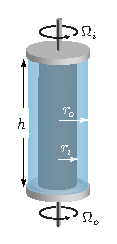
\includegraphics[width=.15\columnwidth]{Figures/1_Apparatus.eps}
    \caption{(a) A schematic diagram of the experimental system.}\label{fig:schematic}
\end{figure}

\section{Apparatus}

Figure \ref{fig:schematic} is a schematic representation of a TC cell. The following is a list of the important parameters for a TC cell along with the values for the system described in detail in the mechanical drawings in the appendix. Note that these values can be varied but the details of the fluid dynamics will be different than we describe:
\begin{itemize}
\item Inner cylinder radius, $a = 3.07$ cm
\item Outer cylinder radius, $b = 3.49$ cm
\item Radius ratio, $a/b = 0.880 $
\item Gap between cylinders, $d = b-a = 0.419$ cm
\item Inner cylinder rotation frequency, $f_{cyl}$
\item Outer cylinder rotation frequency = 0  (in the general problem the outer cylinder as well as the inner cylinder rotates)
%\item Kinematic viscosity of water at 20.0 deg Celsius, $\nu = 0.01000$ cm$^2$/s
%\item Kinematic viscosity of water at 27.5 deg Celsius, $\nu = 0.00845$ cm$^2$/s
%\item Reynolds number, $R =(2\pi f_{cyl} a) d/\nu$
\item Annulus height, $H= 8.38$ cm, set by annular rings at ends
\item Aspect ratio, $H/d = 20.0$

\end{itemize}
Our system is made using acrylic sheets for the top and bottom lids and stock acrylic cylinders for the inner and outer cylinders. Brass and aluminum could also be used for the top and bottom lids of the system and for the inner cylinder though the cost would be higher.

We use a very low-cost technique for flow visualization based on the work of Borrero et a. \cite{borrero_2018}. The authors describe a simple technique to extract stearic acid crystals from shaving cream. These crystals are highly reflective and flat so they preferentially align themselves in the shear direction, which makes them ideal for visualizing the instabilities in a TC cell.

\section{Hands-on observations}
In this section we describe the activities used at the Hands-On School in Complex Systems, which have been optimized by Harry Swinney and Bruce Rodenborn over the past 12 years. The students work in groups of four to six in a three-hour session. The students at the Hands-On School are typically post-doctoral researchers or junior faculty in developing countries. However, they generally have little experience with fluid dynamics or nonlinear dynamics. Thus, the program we describe can be easily adapted to suit the level of a given class.

\begin{figure}[ht]
  \centering
    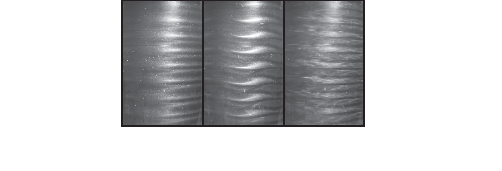
\includegraphics[width=.75\columnwidth]{Figures/2_Flow_Images.eps}
    \caption{Couette-Taylor flow instabilities showing the sequence of instabilities for increasing values of $f_{cyl}$: (a) Taylor vortices (b) wavy vortices (c) turbulent Taylor vortices.}\label{fig:flow_patterns}
\end{figure}

\subsection{The base flow state}
The learning goals here are: ...
Students are given a brief introduction to the TC cell and asked to describe what they believe are its relevant parameters. This generally leads to a lively discussion of how to characterize the system and the fluid flow. We also introduce the Reynolds number, which is a dimensionless parameter common in fluid dynamics defined as:

\BE
Re\equiv \frac{Lv}{\nu},
\EE
where $L$ is a typical length scale in the system, often taken to be the gap width $d$, $v$ is a typical velocity scale in the system, the tangential velocity of the inner cylinder $v=2\pi f_{cyl}a$, and $\nu$ is the kinematic viscosity of the fluid, which for water is $\nu\approx 0.01~\rm cm^2/ s$  \cite{fluids_general}.

The introduction of the Reynolds provides the opportunity to discuss dimensions versus units in physics and fluids, and it allows for a discussion of Reynolds number scaling, whereby different sized systems will display the same flow dynamics if the Reynolds number is held constant between them \cite{fluids_general}.

The students are then given the equation for the laminar base flow, where fluid parcels move in circles at different velocities depending on their location within the gap: 
\BE
v_\phi = Ar + B/r
\label{eq:base_flow}
\EE
(Deriving this solution could be part of a course in fluid dynamics so the work here would be the culmination of the analytical analysis of the TC cell done prior to the experimental phase.) We discuss the unique solution of the Navier-Stokes equations for our system, which involves a discussion of boundary value problems and a discussion of the proper boundary conditions for laminar fluid flow. The students are allowed to consider what would be appropriate and G.I. Taylor's work is introduced, which first made clear that no-slip boundary conditions are the best model for laminar fluid flow. Students can then determine the unique values for $A$ and $B$ in Eq.(\ref{eq:base_flow}) though this work is not essential for what follows. 

\subsection{Onset of Taylor vortex flow: instability of the laminar base flow}

The next phase of the experiment requires the students to experimentally determine the rotation rate $f_{\rm cyl}$ at which the base flow state becomes unstable. The critical cylinder rotation rate $(f_{cyl})_c$ for the onset of Taylor vortex flow is measured in observations of spatial patterns made visible by suspending the stearic acid crystals into the fluid, see Fig. \ref{fig:flow_patterns}  The work has two pedagogical goals. The first is to see and understand how a dynamical system transitions from one flow state to a more complicated motion. The second goal is to develop a methodology for searching in a parameter space for a transition. This discussion described as being much broader than the work on the TC cell. It might be the analysis of computational results or chemical reaction where a single parameter is varied to determine the onset of a change in the dynamics of a system. This type of search is common in many scientific disciplines. 

Students are asked to increase the rotation rate from the laminar state to near maximum, which is where the fluid is turbulent. They are thus aware of a rotation rate value where the laminar solution is correct and another value where the laminar solution is clearly not correct. The group is asked to determine the optimal choice for the next rotation rate to most quickly determine the onset of the Taylor vortex instability. If more than one group is present, the task is presented as a challenge to incentivize  collaboration and to think about efficiently finding the transition rotation rate $(f_{cyl})_c$.

The students are given the following tasks and asked to answer the associated questions:
\begin{enumerate}
%\item  Learn how to set motor speed and acceleration rate  (see Instrumentation: Motor Control). 
\item  Increase the cylinder rotation frequency from rest until Taylor vortices are observed to form.  Do the vortices emerge in the middle or at the ends, or everywhere simultaneously? Why? 
\item  Work as a team to determine $(f_{cyl})_c$ by picking a sequence of values of 
$f_{cyl}$ below and above the Taylor instability onset.  See how quickly you can determine a value of $(f_{cyl})_c$ that you estimate has an uncertainty less than 2\%. 
\item Is there hysteresis in the transition from laminar flow to Taylor vortex flow? That is, does the transition occur at the same  $(f_{cyl})_c$ value for $f_{cyl}$ increasing and decreasing? (Note that there should be not hysteresis in this transition. The discussion allows for more advanced discussions of different types of nonlinear transitions for students with sufficient background knowledge, c.f. Strogatz \cite{strogatz}.)
\item  How many Taylor vortices are there? That is, what is the axial wavelength $\lambda$ at  $R_c$, given that there are two counter-rotating vortices per axial wavelength?  Compute the axial wavelength in units of the gap $d$ between the cylinders:  $\lambda/d$. Compare your value for $\lambda/d$ with the theoretical prediction, which is $\lambda/d=1$ as predicted by G.I. Taylor \cite{taylor}.
\end{enumerate}
These activities typically take about 30-45 minutes including time for associated discussions. The next task is to find the second transition, which is a time dependent flow state -- wavy vortex flow. The students are already aware of higher order transitions because they saw the system rotating at the maximum rate in the previous search for the first instability in the system.   

\subsection{Wavy vortex flow}

At a critical cylinder rotation rate beyond the onset of the  time-independent Taylor vortex instability, time-dependent traveling waves appear on the Taylor vortices. These beautiful spatial patterns are then analyzed by making digital movies with a web camera, see Fig. \ref{fig:flow_patterns}.

 The students perform an analysis similar to that done by Gollub and Swinney in 1978\cite{gollub_swinney_1978}, which first showed direct evidence of chaos in a dynamical system. The students analyze the time-dependent wavy vortex flow by computing {\it Power Spectra} from {\it Fast Fourier Transforms} of intensity time series data obtained from digital movies.  

At yet higher cylinder speeds, beyond the onset of traveling waves, there are transitions to multi-periodic, chaotic, and finally turbulent flows.  These transitions in the flow dynamics can also be identified and quantified from analyses of  power spectra of the digital movies. However, completing the work in this section along with the previous search and discussions generally takes at least three hours so the Hand-On students rarely complete more than an initial power spectrum. Students have returned for an additional three hour session to explore these dynamics.

The following are the instructions given to students to quantify the wavy flow state they are observing:

\begin{enumerate}
\item {\bf Observe wavy vortices and measure the wave frequency}: Increase $f_{cyl}$ above the onset of Taylor vortices until traveling azimuthal waves have formed on the Taylor vortices$f_{cyl}\approx 3_1$. . These oscillations are standing waves in the frame moving with at the wave speed. Students are instructed to estimate the frequency $f_1$ of the traveling waves by observing the time for twenty waves to pass a point with $f_{cyl}$ approximately twice the value obtained for the onset of Taylor vortex flow. They time the oscillations so that they have a sense of the timescale for the instability before using a camera and a computer to determine the frequency precisely. This work includes a useful general discussion about using the results of the simplest measurement technique available as a check on the results from a more complicated method of analysis.

\item {\bf Find the azimuthal wavenumber}:  Students estimate  the mode number $m$ for the azimuthal waves by visual observation; that is, if they could stop the motion of the waves and walk all the way round the cylinder, how many waves would they count?

\end{enumerate}

\subsection{Quantifying the dynamics using movies and power spectra}% (see Instrumentation: Camera Operation)}
The students have completed the initial analysis of the wavy vortex flow state and are directed to use a webcam and MATLAB to analyze the flow state more quantitatively. Before recording movies, we discuss various considerations in capturing images of the flow state. The frame rate of the camera is of particular interest. Even inexpensive webcams typically can capture movies in HD formats at frame rates as high as 60 fps. However, the flow state has a typical period of about one second as determined in the previous work. Thus, a high frame rate is probably not necessary, which includes a discussion of the Nyquist theorem in spectral theory \cite{nyquist}. We also discuss typical considerations in performing a fast Fourier transform (FFT) of a temporal signal and the broad applicability of FFT's in temporal and spatial analyses.

Other considerations are exposure (integration time),  contrast, etc. so the experiment requires students to consider scientific images in a different way than more casual photography. For instance, we discuss the dynamic range of the camera and how digital images are captured. We stress that the images spanning the range of the 8-bit camera capture the most information so the video should be neither under nor over exposed. The discussion includes many other aspects of scientific videography and is a great primer for those that have never used a digital camera for science.

These experiments also provide a direct opportunity to see how noise in a signal affects measurements and how averaging can eliminate random error. Here, each pixel is considered an independent measurement of the intensity scattered from the fluid. However, each of these signals contains noise from the cameras CCD and other random sources. The computer algorithm requires user input to select a region of the image for analysis. Even a small region of a 640x480 image will include $\sim 10^3$ pixels. The algorithm computes the averaged power spectral density from these pixels and displays the average spectrum along with a randomly chosen single pixel's spectrum, which will show higher levels of noise and may not show any of the fundamental frequencies in the flow. 

The following are the subjects described in the handout given to the participants:
\begin{enumerate}

\item {\bf Frame rate for movie}:  By the Nyquist theorem, the maximum frequency of a spectrum is one-half the sampling rate. Therefore, the movie frame rate should be at least $2f_1$. In order to increase confidence in the interpretation of the spectra, choose a frame rate fast enough so a spectrum will include the second and third harmonics; that is, choose a frame rate somewhat greater than $6f_1$.

\item {\bf Movie duration}:  The width of a peak [full width at half maximum (FWHM)] in a power spectrum corresponding to a sinusoidal signal is approximately $1/T$, where $T$ is the duration of the data set (length of the movie).  For accurate characterization of the dynamics, the characteristic frequency should be determined to 1\%. Hence the FWHM should be only $1\%$ of the component frequency $f_1$, which means the duration $\Delta t$ of the movie should be at approximately $\Delta t=100T$.  
\item {\bf Aliasing}:   Compare two movies recorded with different frame rates, say one with frame rate about $7f_1$ and another with frame rate about $20f_1$.  What differences do you see in the spectra?  Ask the instructor to discuss aliasing:  a spectral component $f*$ that is undersampled will fold back into the spectrum giving a component at  $2f_{\rm NYQUIST} - f*$.


\item {\bf Signal to noise}:  Spectral noise can be reduced by averaging many spectra.  Compare for two cases the signal-to-noise ratio for spectra made from the same movie, where the signal-to-noise is given by the ratio of the signal power for the fundamental spectral component $P(f_1)$  to the background noise $P(f)$:  (1) a spectrum computed by averaging the spectra from about 50 pixels, and (2) a spectrum computed by averaging the spectra from about 10000 pixels.  What do you conclude?

\end{enumerate}

\section{Higher instabilities:  multi-periodicity, chaos, and turbulence} 
\subsection{Modulated wavy vortex flow: flow with two incommensurate characteristic frequencies}


With increasing Reynolds number there are further instabilities characterized by power spectra that become too complex to analyze in detail in a three hour laboratory session.  However, students that return for a second session complete some or all of the activities described below. The exercises use several classic techniques from nonlinear dynamics and chaos theory. Thus, it makes it an ideal complement to a course or module in nonlinear dynamics, which often lack good physical examples of theory.

\begin{enumerate}

\item \textbf{Modulated waves and chaos:} With an increase in $Re$ for a wavy vortex state, at some larger $Re$, typically $12( f_{cyl})_c$, a second characteristic frequency $f_2$ will appear in the power spectrum. This modulated wavy vortex flow is composed of two traveling waves with different azimuthal wavenumbers that also have different wave speeds. The Taylor vortex pattern is then time dependent even in the co-rotating frame of the original wavy vortices.  The frequency $f_2$ corresponds to an azimuthal traveling wave similar to the wavy vortices; the angular speed of the modulated waves is about $v_{\rm wave}\approx0.44f_{cyl}$, and typically the number $m_2$ of the secondary waves around the annulus is 4, resulting in $f_2 \approx 4\times v_{\rm wave}= 1.76 f_{cyl}$.  

Students are instructed to accelerate the inner cylinder slowly from rest at 0.01 rev/sec$^2$ to a rotation rate of $f_{cyl}=$1.68 Hz. We discuss the qualitative difference between the power spectrum for this flow and the spectrum for the wavy vortex flow observed earlier at $f_{cyl}$= 0.3 Hz. The two frequency spectrum is much more complicated (Fig. XX) because it includes linear sums of the two fundamental frequency, whereas the figure shows the relatively simple ``picket fence'' spectrum of a singly periodic flow state. 



\begin{enumerate}
\item  Start with a wavy vortex flow state with four waves at about $Re=8R_c$.  Increase $Re$ slowly until a second characteristic frequency $f_2$ appears in the power spectrum.  
\item  Observe the effect of the modulation on the waves in the movies. Students will observe constructive and destructive interference between the two traveling waves.
\item  Commensurate and incommensurate frequencies can never be distinguished experimentally, but it is possible to obtain strong experimental evidence for incommensurability.  Students are asked to develop a test for obtaining such evidence. They are guided to finding what they consider to be the fundamental frequencies in the flow and then taking the ratio to show that, within the uncertainty of the experiment, the frequencies are irrationally related.
\item The final task is to increase the cylinder rotation rate to $\sim$4 Hz and obtain and interpret a power spectrum, Fig. XXX.c.  The spectrum shows no distinct peaks and a much higher noise level than the previous spectra. They are also asked to look at the movies frame by frame and discuss the fluid's behavior, which now shows significantly more fine scale motion. Time permitting, the students  also capture power spectra in the range $1.68 {\rm ~Hz} <f_{cyl}<4$ Hz and see the noise floor in the spectrum rise to swamp the frequencies in the fluid.
\end{enumerate}
\end{enumerate}


\subsection{Phase space portraits}

An $n$-dimensional phase space for a dynamical system can be constructed from vectors obtained from a time series for a single variable $x(t)$ by using the method of time delays, where a point in the space is given by $X(t)$ = $\{x(t), x(t-\tau), x(t-2\tau), . . .  \ , x(t-(n-1)\tau)\}$. The phase portrait characterizing the dynamics is given by the trajectory $X(t)$ in the $n$-dimensional phase space.  For a $d$-dimensional attractor an embedding in the phase space is assured if $n > 2d$ by the Takens embedding theorem (1981), which is a generalization of the Whitney embedding theorem (1936); see Roux, Simoyi, $\&$ Swinney, Physica D 8, 257 (1983).

\begin{enumerate}
\item The GUI program saves the pixels selected for analysis as a data file, which the students can read back into MATLAB. They construct the phase space attractors for a flow with one fundamental frequency (limit cycle attractor) and for a flow with two incommensurate characteristic frequencies (a 2-torus attractor) using the averaged pixel data, Fig. XXX (appendix?).
\item They then construct the phase space portrait for a case where the power spectrum includes broadband noise in addition to sharp characteristic frequencies and create figures similar to Fig. 6 in Brandstater et al. \cite{brandstater_et_al_1987}.
\end{enumerate}

\subsection{Chaos, Strange Attractors, Lyapunov exponents, fractal dimension, turbulence}

The largest Lyapunov exponent characterizes the exponential rate of separation in phase space of two points that were initially infinitesimally separated.  A system is chaotic if the largest Lyapunov exponent is positive.  In practice the fractal dimension and Lyapunov exponent spectrum can be determined from laboratory observations only for systems whose dynamics is characterized by a low dimensional phase space attractor; the number of data points needed increases roughly as $\approx$10$d$.  However, the concept of Lyapunov exponents can be very useful even for strongly turbulent flows that have coherent structures (jets and vortices). A turbulent flow is characterized not only by sensitive dependence on initial conditions (the defining property of chaos), but also by a large range in spatial and temporal scales. The scaling of turbulence in concentric cylinder systems has been studied for Reynolds numbers up to $\sim10^6$.   It is difficult to go to higher $Re$ in controlled laboratory experiments because of Joule heating due to the stirring by differential rotation of the cylinders; the power dissipation with water as a working fluid can easily be kilowatts when the Reynolds number is $Re\sim10^6$.

The first direct observation of chaos in a dynamical system was by Gollub and Swinney in 1978 \cite{gollub_swinney}. Students can repeat their work by studying changes in the spectral signal measured with the webcam. The system will display a sequence of instabilities that include two incommensurate frequencies, but after the second time dependent instability, no additional frequencies appear in the system. Instead, the signal shows a rapid increase in the noise floor, which rises until it swamps the two frequencies that first appear. The noisiness results from fine scale motion within the Taylor vortex boundaries that persist to high rotation rates of the inner cylinder.


\section{Methods}\label{sec:methods}



\section{ Results }\label{sec:results}

\section{ discussion } \label{sec:discussion}


\end{document}



%
% ****** End of file apssamp.tex ******}